% !TEX program = xelatex
% c5p-s-2026-final.tex
% 2026 €€£ 超专业级别硬件能力认证第一轮（C5P-S1）提高级 C++语言试题（模拟卷）
% 版式：a4paper、等线题头、宋体中文 + Consolas 西文、页脚两行（PDF 格式）、选项每行一个、大题强制换页
% 代码：带边框、左侧行号 0 补齐、无横向线条；阅读程序不写概要，完善程序写概要后挖空
% 编译方式：xelatex c5p-s-2026-final.tex（建议编译两次）
\documentclass[a4paper]{ctexart}

\usepackage{fontspec}
\usepackage{graphicx}
\usepackage{tikz}
\usetikzlibrary{arrows.meta}
\usepackage{eso-pic}
\newcommand{\waterword}{%
  \makebox[0pt][c]{%
    \tikz[baseline]{%
      \node[
        inner sep=0pt,
        rotate=-35,
        text=black,
        opacity=0.085,
        font=\fontsize{54}{70}\selectfont
      ] {折工};%
    }%
  }%
}
\AddToShipoutPictureFG{%
  \put(\LenToUnit{-0.3cm},\LenToUnit{1.2cm}){\waterword}%
  \put(\LenToUnit{5.0cm},\LenToUnit{0.0cm}){\waterword}%
  \put(\LenToUnit{10.3cm},\LenToUnit{1.4cm}){\waterword}%
  \put(\LenToUnit{15.6cm},\LenToUnit{0.2cm}){\waterword}%
  \put(\LenToUnit{2.2cm},\LenToUnit{6.2cm}){\waterword}%
  \put(\LenToUnit{7.5cm},\LenToUnit{4.8cm}){\waterword}%
  \put(\LenToUnit{12.8cm},\LenToUnit{6.3cm}){\waterword}%
  \put(\LenToUnit{18.1cm},\LenToUnit{4.9cm}){\waterword}%
  \put(\LenToUnit{-0.3cm},\LenToUnit{10.0cm}){\waterword}%
  \put(\LenToUnit{5.0cm},\LenToUnit{11.5cm}){\waterword}%
  \put(\LenToUnit{10.3cm},\LenToUnit{10.1cm}){\waterword}%
  \put(\LenToUnit{15.6cm},\LenToUnit{11.6cm}){\waterword}%
  \put(\LenToUnit{2.2cm},\LenToUnit{16.5cm}){\waterword}%
  \put(\LenToUnit{7.5cm},\LenToUnit{15.1cm}){\waterword}%
  \put(\LenToUnit{12.8cm},\LenToUnit{16.6cm}){\waterword}%
  \put(\LenToUnit{18.1cm},\LenToUnit{15.2cm}){\waterword}%
  \put(\LenToUnit{-0.3cm},\LenToUnit{21.6cm}){\waterword}%
  \put(\LenToUnit{5.0cm},\LenToUnit{23.1cm}){\waterword}%
  \put(\LenToUnit{10.3cm},\LenToUnit{21.7cm}){\waterword}%
  \put(\LenToUnit{15.6cm},\LenToUnit{23.2cm}){\waterword}%
  \put(\LenToUnit{2.2cm},\LenToUnit{27.3cm}){\waterword}%
  \put(\LenToUnit{7.5cm},\LenToUnit{25.9cm}){\waterword}%
  \put(\LenToUnit{12.8cm},\LenToUnit{27.4cm}){\waterword}%
  \put(\LenToUnit{18.1cm},\LenToUnit{26.0cm}){\waterword}%
}
\usepackage{geometry}
\geometry{top=2.7cm, left=2.7cm, right=2.7cm, bottom=4cm}
\setmainfont{Consolas}
\setmonofont{Consolas}
\setCJKmainfont{SimSun}
\newCJKfontfamily{\dengxian}{DengXian}

\usepackage{fancyhdr}
\usepackage{lastpage}
\usepackage[most]{tcolorbox}
\usepackage{listings}
\usepackage{enumitem}
\usepackage{amsmath}
\usepackage{xcolor}
\DeclareMathSizes{10.53937}{10.95}{7.5}{5.5}

% 将带圈数字 ①-⑤ 划入 CJK 字符类，确保题干“①处应填”用中文字体正常渲染
\xeCJKDeclareCharClass{CJK}{"2460 -> "2464}

% ---------------- 页脚：中文宋体 + 数字英文 Times New Roman（参考 cspjs2024hs.pdf 样式） ----------------
\newfontfamily\trm{Times New Roman}
% 普通 Unicode 黑圆点，避免依赖 Wingdings 私有字形映射
\newcommand{\wdot}{{\fontsize{12}{12}\selectfont\textbullet}}
\pagestyle{fancy}
\fancyhf{}
\setlength{\footskip}{1.5cm}
\fancyfoot[C]{{\xeCJKsetup{CJKecglue={\hskip0pt}}{\trm €€£ C5P-S 2026 }{\songti 第一轮 }{\trm C++}{\songti 语言试题}}\\[2pt]{\xeCJKsetup{CJKecglue={\hskip0pt}}{\songti 第}{\trm\thepage}{\songti 页，共}{\trm\pageref{LastPage}}{\songti 页}}}
\renewcommand{\headrulewidth}{0pt}
\renewcommand{\footrulewidth}{0pt}

% ---------------- 代码样式：框宽 14cm、Consolas 12pt、行号 8.5pt(约0.3cm高)、关键字不加粗 ----------------
\renewcommand{\thelstnumber}{\ifnum\value{lstnumber}<10 0\fi\arabic{lstnumber}}
\lstset{
  language=C++,
  basicstyle=\ttfamily\fontsize{12}{14.4}\selectfont,
  numberstyle=\ttfamily\fontsize{12}{14.4}\selectfont\makebox[0.92cm][r],
  numbers=left,
  numbersep=0.08cm,
  frame=none,
  framesep=6pt,
  rulecolor=\color{black!70},
  columns=fullflexible,
  keepspaces=true,
  aboveskip=0pt,
  belowskip=0pt,
  xleftmargin=0.88cm,
  linewidth=13cm,
  showstringspaces=false,
  breaklines=true,
  breakatwhitespace=false,
  keywordstyle=\ttfamily,
  commentstyle=\ttfamily,
  stringstyle=\ttfamily,
  escapeinside={|@}{@|},
}

% 代码框：线1（左框线）距页左 2.05cm；行号列线1→线2 严格 1cm；代码列线2→线3 严格 13cm；
% 线3（右框线）距页右约 4.95cm（A4 宽 21cm 自动吻合）；挖空下划线 2.10cm + 居中序号
\newtcolorbox{codebox}{enhanced, breakable, sharp corners, boxrule=0.5pt, colframe=black, colback=white,
  width=13.45cm, left skip=-0.65cm, before skip=6pt, after skip=8pt,
  top=2pt, bottom=2pt, left=0pt, right=0pt,
  overlay={\draw[black,line width=0.5pt] ([xshift=1.0cm]frame.north west)--([xshift=1.0cm]frame.south west);}}
% 完善程序挖空：2.10cm 下划线 + 居中序号（字体同代码 12pt）
\newcommand{\blank}[1]{\underline{\makebox[2.1cm][c]{#1}}}

\setlength{\parindent}{0pt}
\setlength{\parskip}{2pt}
\linespread{1.25}

% 大题标题（左对齐黑体）
\newcommand{\bigtitle}[1]{\noindent\heiti #1\par\vspace{2pt}}
% 小题题干（序号数字不加粗，Consolas）
\newcommand{\q}[1]{\noindent #1}
% 阅读程序小题：题号前加 Unicode 黑点（整体左对齐）
\newcommand{\qdot}[1]{\noindent\wdot\hspace{0.6em}#1}
% 单个选项（每个选项独立一行）
\newcommand{\opt}[1]{\hspace*{2em} #1\par}
% 完善程序选项：两个选项一行（A B 一行、C D 一行）
\newcommand{\optw}[2]{\hspace*{2em} #1\hspace*{2em}#2\par}

\begin{document}

\begin{center}
{\dengxian
{\xeCJKsetup{CJKecglue={\hskip 0.419em}}\fontsize{15.95}{1}\selectfont 2026 €€£超专业级别硬件能力认证第一轮} \\[1.5em]
    {\xeCJKsetup{CJKecglue={\hskip 0.419em}}\fontsize{15.95}{1}\selectfont （C5P-S1） 提高级 C++\hspace{0pt}语言试题} \\[1.5em]
{\xeCJKsetup{CJKecglue={\hskip 0.344em}}\fontsize{14.05}{1}\selectfont 认证时间：2026年9月18日14:30\textasciitilde16:30}
}
\end{center}

\vspace{8pt}
\noindent{\heiti 考生注意事项：}
\begin{itemize}[leftmargin=2.6em, itemsep=1pt, label={}]
  \item \wdot\hspace{0.5em}试题纸共有 \pageref{LastPage} 页，答题纸共有 1 页，满分 100 分。请在答题纸上作答，写在试题纸上的一律无效。
    \item \wdot\hspace{0.5em}不得使用任何电子设备（如计算器、手机、电子词典等）或查阅任何书籍资料。
\end{itemize}

\bigtitle{一、单项选择题（共 15 题，每题 2 分，共计 30 分；每题有且仅有一个正确选项）}
\q{1.} 下列 Linux 命令中，用于连接并显示文件内容的是（\qquad）\\
\opt{A. \texttt{cp}}\opt{B. \texttt{cat}}\opt{C. \texttt{ping}}\opt{D. \texttt{touch}}
\q{2.} 已知某用二叉链表存储的哈夫曼树共有 \texttt{m} 个叶子结点，则该哈夫曼树中总共有多少个空指针域（\qquad）\\
\opt{A. \texttt{m}}\opt{B. \texttt{m+1}}\opt{C. \texttt{2m}}\opt{D. \texttt{2m+1}}
\q{3.} 对于一棵包含 \texttt{n} 个结点的完全二叉树，对每个叶子结点向上访问直到根结点，统计路径上经过的结点数之和。总时间复杂度为（\qquad）\\
\opt{A. \texttt{O(n)}}\opt{B. \texttt{O(n log n)}}\opt{C. \texttt{O(n\^{}2)}}\opt{D. \texttt{O(n\^{}2 log n)}}
\q{4.} 小 h 从原点 \texttt{(0,0)} 出发，每一步向右或向上走，到达点 \texttt{(5,5)}，且始终满足 \texttt{x >= y}。满足条件的路径有多少条（\qquad）\\
\opt{A. 252}\opt{B. 90}\opt{C. 132}\opt{D. 42}
\q{5.} 用两个栈模拟一个队列，入队时元素统一压入栈 A。正确的出队操作是（\qquad）\\
\opt{A. B 为空时将 A 全部转移到 B，再从 B 弹出；B 非空时直接从 B 弹出}
\opt{B. 无论 B 是否为空，都先将 A 全部转移到 B，再从 B 弹出}
\opt{C. 直接删除 A 的栈底元素}\opt{D. 直接从 A 弹出栈顶元素}
\q{6.} 从集合 \texttt{\{1,2,3,4,5,6,7,8,9,10\}} 中选出 4 个不同的数，要求任意两个被选数都不相邻。不同的选法共有（\qquad）\\
\opt{A. 15}\opt{B. 20}\opt{C. 35}\opt{D. 70}
\q{7.} 在 C++ 中，关于 \texttt{std::set<int>} 与 \texttt{std::map<int, int>} 的说法，正确的是（\qquad）\\
\opt{A. \texttt{set} 中的元素可以重复}\opt{B. \texttt{map} 按插入顺序存储键值对}
\opt{C. \texttt{set} 自动有序，插入、删除、查找复杂度均为 \texttt{O(log n)}}\opt{D. \texttt{map} 的键可以重复}
\q{8.} 关于有向无环图的拓扑排序，下列说法正确的是（\qquad）\\
\opt{A. 任何有向无环图的拓扑排序都唯一}\opt{B. 含有环的有向图也可以进行拓扑排序}
\opt{C. 若有边 \texttt{u -> v}，则任一拓扑序中 \texttt{u} 在 \texttt{v} 之前}\opt{D. 拓扑排序就是深度优先遍历序列}
\q{9.} KMP 算法中，\texttt{next} 数组的主要作用是（\qquad）\\
\opt{A. 记录模式串失配后应回溯到的位置}\opt{B. 记录主串每个字符出现的次数}
\opt{C. 记录主串的后缀数组}\opt{D. 与模式串无关地跳过主串位置}
\q{10.} 对一个 \texttt{n} 个顶点、\texttt{m} 条边的带权有向图使用不带堆优化的 Dijkstra 算法，时间复杂度为（\qquad）\\
\opt{A. \texttt{O(n\^{}2)}}\opt{B. \texttt{O(m log n)}}\opt{C. \texttt{O((m+n) log n)}}\opt{D. \texttt{O(mn)}}
\q{11.} 已知 20260913 是质数，表达式 \texttt{(1/2 + 1/3 + ... + 1/20260912)\^{}20260913 mod 20260913} 的值为（\qquad）\\
\opt{A. 0}\opt{B. 1}\opt{C. \texttt{2\^{}20260913 mod 20260913}}\opt{D. 20260912}
\q{12.} 设 \(p=20260913\) 为质数。在模 \(p\) 意义下，
\[
\sum_{i=1}^{p-2}\frac{1}{i(i+1)}
\]
等于（\qquad）\\
\opt{A. 0}\opt{B. 1}\opt{C. 2}\opt{D. \(p-2\)}

\q{13.} 对下图恰好删去两条不同的边，使得仍存在从 1 到 8 的有向路径。删边方案共有（\qquad）种
\begin{center}
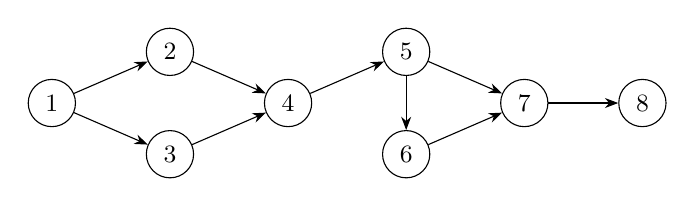
\begin{tikzpicture}[>=Stealth, every node/.style={circle, draw, fill=white, minimum size=6mm, inner sep=0.5pt, font=\small}]
  \node (n1) at (0,0) {1}; \node (n2) at (1.5,0.65) {2}; \node (n3) at (1.5,-0.65) {3};
  \node (n4) at (3,0) {4}; \node (n5) at (4.5,0.65) {5}; \node (n6) at (4.5,-0.65) {6};
  \node (n7) at (6,0) {7}; \node (n8) at (7.5,0) {8};
  \draw[->] (n1)--(n2); \draw[->] (n1)--(n3); \draw[->] (n2)--(n4); \draw[->] (n3)--(n4);
  \draw[->] (n4)--(n5); \draw[->] (n5)--(n6); \draw[->] (n5)--(n7); \draw[->] (n6)--(n7); \draw[->] (n7)--(n8);
\end{tikzpicture}
\end{center}
\opt{A. 12}\opt{B. 15}\opt{C. 18}\opt{D. 21}

\q{14.} 1 到 200 之间，不能被 2、3、7 中任何一个整除的整数共有（\qquad）个\\
\opt{A. 57}\opt{B. 58}\opt{C. 59}\opt{D. 60}
\q{15.} 已知如下 C++14 代码定义 Ackermann 函数：
\begin{codebox}\begin{lstlisting}
long long A(int m, long long n) {
    if (m == 0) return n + 1;
    if (n == 0) return A(m - 1, 1);
    return A(m - 1, A(m, n - 1));
}
\end{lstlisting}\end{codebox}
则 \(A(2,3)\) 的值为（\qquad）\\
\opt{A. 5}\opt{B. 7}
\opt{C. 9}\opt{D. 13}

\clearpage
\bigtitle{二、阅读程序（程序输入不超过数组或字符串定义的范围；判断题正确填√，错误填×；除特殊说明外，判断题 1.5 分，选择题 3 分，共计 40 分）}

\noindent（1）给定一个非空字符串，程序先求出每个前缀的最长真前缀与后缀公共长度，
再把整个字符串以及它的各级相同前后缀的长度相加并输出。输入字符串只含小写英文字母。
\begin{codebox}\begin{lstlisting}
#include <bits/stdc++.h>
using namespace std;
const int N = 2e5 + 5;
int n, pi[N];
string s;

int main() {
    cin >> s;
    n = s.size();
    for (int i = 1; i < n; ++i) {
        int j = pi[i - 1];
        while (j && s[i] != s[j]) j = pi[j - 1];
        if (s[i] == s[j]) ++j;
        pi[i] = j;
    }
    int ans = 0;
    for (int len = n; len > 0; len = pi[len - 1]) ans += len;
    cout << ans << '\n';
}
\end{lstlisting}\end{codebox}

\noindent\wdot\hspace{0.5em}判断题\\
\q{16.} 对 \(0\le i<n\)，\texttt{pi[i]} 等于 \texttt{s[0..i]} 的最长真前缀与后缀的公共长度。（\qquad）\\
\opt{A. 正确}\opt{B. 错误}
\q{17.} 若把累加长度循环的初始化语句 \texttt{len = n} 改为 \texttt{len = pi[n-1]}，则对任意输入，程序输出都恰好减少 \texttt{n}。（\qquad）\\
\opt{A. 正确}\opt{B. 错误}
\q{18.} 若把求解 \texttt{pi} 的循环中的 \texttt{while} 改成 \texttt{if}，则对所有输入，程序输出仍然不变。（\qquad）\\
\opt{A. 正确}\opt{B. 错误}

\noindent\wdot\hspace{0.5em}单选题\\
\q{19.} 输入 \texttt{abacababacabab} 时，程序输出为（\qquad）\\
\opt{A. 16}\opt{B. 20}\opt{C. 24}\opt{D. 28}
\q{20.}（4 分）若输入字符串长度为 $n$，且字符比较、数组访问均视为 $O(1)$，则程序的最坏时间复杂度和空间复杂度分别为（\qquad）\\
\opt{A. 时间 $O(n^2)$，空间 $O(n)$}
\opt{B. 时间 $O(n)$，空间 $O(n)$}
\opt{C. 时间 $O(n\log n)$，空间 $O(\log n)$}
\opt{D. 时间 $O(n^2)$，空间 $O(1)$}

\noindent（2）给定一个有 \texttt{n} 行、\texttt{m} 列的棋盘，字符 \texttt{\#} 表示不能放置，
其余位置可以放置。要求同一行相邻位置、相邻两行同一列的位置不能同时放置，程序求合法方案数。
\begin{codebox}\begin{lstlisting}
#include <bits/stdc++.h>
using namespace std;
const int P = 998244353, M = 10;
int n, m, ban[105], f[2][1 << M];
vector<int> st;

int main() {
    cin >> n >> m;
    for (int i = 1; i <= n; ++i) {
        string s; cin >> s;
        for (int j = 0; j < m; ++j)
            if (s[j] == '#') ban[i] |= 1 << j;
    }
    for (int s = 0; s < (1 << m); ++s)
        if ((s & (s << 1)) == 0) st.emplace_back(s);
    f[0][0] = 1;
    for (int i = 1; i <= n; ++i) {
        int pre = i & 1, cur = pre ^ 1;
        int mask = pre ^ cur;
        pre ^= mask;
        cur ^= mask;
        memset(f[cur], 0, sizeof(f[cur]));
        for (auto&& s : st) {
            if (s & ban[i]) continue;
            for (auto&& t : st) {
                if (s & t) continue;
                f[cur][s] += f[pre][t];
                if (f[cur][s] >= P) f[cur][s] -= P;
            }
        }
    }
    int ans = 0;
    for (auto&& s : st) {
        ans += f[n & 1][s];
        if (ans >= P) ans -= P;
    }
    cout << ans << '\n';
}
\end{lstlisting}\end{codebox}

\noindent\wdot\hspace{0.5em}判断题\\
\q{21.} 表达式 \texttt{(s \& (s << 1)) == 0} 的作用是筛掉同一行中相邻列同时被选中的状态。（\qquad）\\
\opt{A. 正确}\opt{B. 错误}
\q{22.} 处理第 \(i\) 行时，若 \texttt{s} 表示当前行状态、\texttt{t} 表示上一行状态，则条件 \texttt{if (s \& t) continue} 保证相邻两行的同列位置不会同时被选中。（\qquad）\\
\opt{A. 正确}\opt{B. 错误}
\q{23.}（2 分）若删去每轮开始时的 \texttt{memset(f[cur], 0, sizeof(f[cur]))}，则程序对所有输入的输出仍不变。（\qquad）\\
\opt{A. 正确}\opt{B. 错误}

\noindent\wdot\hspace{0.5em}单选题\\
\q{24.} 记 \(V=\texttt{st.size()}\)，则程序的时间复杂度为（\qquad）\\
\opt{A. \(O(nV)\)}\opt{B. \(O(nV^2+2^m)\)}\opt{C. \(O(n2^{2m})\)}\opt{D. \(O(n^2V)\)}
\q{25.} 输入为 \texttt{n=2,m=3}，两行均为 \texttt{...} 时，程序输出为（\qquad）\\
\opt{A. 15}\opt{B. 16}\opt{C. 17}\opt{D. 18}
\q{26.} 在处理第 \(i\) 行之前，若 \texttt{s} \(\in\) \texttt{st}，则 \texttt{f[pre][s]} 表示（\qquad）\\
\opt{A. 前 \(i\) 行中最后一行状态为 \texttt{s} 的合法方案数}
\opt{B. 前 \(i-1\) 行中最后一行状态为 \texttt{s} 的合法方案数}
\opt{C. 长度为 \texttt{m} 的合法行状态总数}
\opt{D. 第 \(i\) 行所有可选位置的数量}

\noindent（3）给定一个长度为 \texttt{n} 的数组，操作 1 \texttt{l r k b} 把区间内每个数变为
\(kx+b\)，操作 2 \texttt{l r} 输出区间和。所有区间下标均合法。
\begin{codebox}\begin{lstlisting}
#include <bits/stdc++.h>
using namespace std;
using ll = long long;
const ll P = 1000000007;
const int N = 2e5 + 5;
int n, q;
ll a[N];
struct Node { ll sum, mul, add; } tr[N << 2];

void build(int p, int l, int r) {
    tr[p].mul = 1;
    if (l == r) { tr[p].sum = a[l] % P; return; }
    int m = (l + r) >> 1;
    build(p << 1, l, m); build(p << 1 | 1, m + 1, r);
    tr[p].sum = (tr[p << 1].sum + tr[p << 1 | 1].sum) % P;
}
void apply(int p, int l, int r, ll k, ll b) {
    tr[p].sum = (tr[p].sum * k + (r - l + 1) * b) % P;
    tr[p].mul = tr[p].mul * k % P;
    tr[p].add = (tr[p].add * k + b) % P;
}
void push(int p, int l, int r) {
    if (l == r) return;
    int m = (l + r) >> 1;
    apply(p << 1, l, m, tr[p].mul, tr[p].add);
    apply(p << 1 | 1, m + 1, r, tr[p].mul, tr[p].add);
    std::exchange(tr[p].mul, 1);
    std::exchange(tr[p].add, 0);
}
void upd(int p, int l, int r, int ql, int qr, ll k, ll b) {
    if (ql <= l && r <= qr) { apply(p, l, r, k, b); return; }
    push(p, l, r);
    int m = (l + r) >> 1;
    if (ql <= m) upd(p << 1, l, m, ql, qr, k, b);
    if (qr > m) upd(p << 1 | 1, m + 1, r, ql, qr, k, b);
    tr[p].sum = (tr[p << 1].sum + tr[p << 1 | 1].sum) % P;
}
ll qry(int p, int l, int r, int ql, int qr) {
    if (ql <= l && r <= qr) return tr[p].sum;
    push(p, l, r);
    int m = (l + r) >> 1;
    ll s = 0;
    if (ql <= m) s = (s + qry(p << 1, l, m, ql, qr)) % P;
    if (qr > m) s = (s + qry(p << 1 | 1, m + 1, r, ql, qr)) % P;
    return s;
}
int main() {
    cin >> n >> q;
    for (int i = 1; i <= n; ++i) cin >> a[i];
    build(1, 1, n);
    while (q--) {
        int op, l, r; cin >> op >> l >> r;
        if (!(op ^ 1)) {
            ll k, b; cin >> k >> b;
            upd(1, 1, n, l, r, k, b);
        } else cout << qry(1, 1, n, l, r) << '\n';
    }
}
\end{lstlisting}\end{codebox}

\noindent\wdot\hspace{0.5em}判断题\\
\q{27.} 同一线段树结点 \texttt{p} 先后执行 \texttt{apply(p,l,r,2,1)}、\texttt{apply(p,l,r,3,4)} 后，其懒标记表示的变换为 \(x\mapsto 6x+7\)。（\qquad）\\
\opt{A. 正确}\opt{B. 错误}
\q{28.} 主函数依次执行两条更新：对区间 \([2,4]\) 先执行 \(x\leftarrow 2x+1\)，再执行 \(x\leftarrow x+3\)。若只交换这两次 \texttt{upd(...)} 调用的先后顺序，最终数组一定不变。（\qquad）\\
\opt{A. 正确}\opt{B. 错误}
\q{29.} 程序的时间复杂度为 \(O((n+q)\log n)\)。（\qquad）\\
\opt{A. 正确}\opt{B. 错误}

\noindent\wdot\hspace{0.5em}单选题\\
\q{30.} 函数 \texttt{apply(p,l,r,k,b)} 执行后，结点 \texttt{p} 中记录的信息应当表示（\qquad）\\
\opt{A. 只把区间左端点变为 \texttt{k*l+b}}
\opt{B. 把区间内每个数都变为 \texttt{k*x+b}，并同步更新区间和及待下传信息}
\opt{C. 只修改两个子结点的区间和，不修改当前结点}
\opt{D. 把区间内每个数都加上 \texttt{k+b}，不再保留乘法信息}
\q{31.} 若把 \texttt{upd} 中递归前的 \texttt{push(p,l,r)} 删除，则下列说法正确的是（\qquad）\\
\opt{A. 只有叶结点上的操作会出错}
\opt{B. 某些部分覆盖更新后再查询时，结果可能出错}
\opt{C. 所有操作的输出都不变，只是速度变慢}
\opt{D. 程序会在第一次更新时立刻停止}
\q{32.}（4 分）初始数组为 \texttt{2 1 3 5 4 6}，依次执行 \texttt{1 2 6 2 1}、\texttt{1 1 4 3 2}、\texttt{1 3 5 1 4}、\texttt{2 2 6}，最后一次操作输出为（\qquad）\\
\opt{A. 97}\opt{B. 101}\opt{C. 103}\opt{D. 107}
\clearpage
\bigtitle{三、完善程序（单选题，每小题 3 分，共计 30 分）}

\noindent（1）（三色序列）给定一个长度为 \texttt{n}、只含字符 \texttt{R,G,Y} 的字符串。每次可以交换两个相邻字符。求使相邻字符均不同所需的最少交换次数；若无法做到，输出 \texttt{-1}。\texttt{1 <= n <= 400}。

\begin{codebox}\begin{lstlisting}
#include <bits/stdc++.h>
using namespace std;
const int N = 405, INF = 1e9;
int n, cnt[3], pos[3][N], pre[3][N];
int f[2][N][N][4];
string s;
int main() {
    cin >> n >> s;
    for (int i = 1; i <= n; ++i) {
        int c;
        if (s[i-1] == 'R') c = 0;
        else if (s[i-1] == 'G') c = 1;
        else c = 2;
        for (int t = 0; t < 3; ++t)
            pre[t][i] = |@\blank{①}@|;
        pos[c][++cnt[c]] = i;
        ++pre[c][i];
    }
    memset(f, 0x3f, sizeof(f));
    f[0][0][0][3] = |@\blank{②}@|;
    for (int len = 0; len < n; ++len) {
        int cur = len & 1, nxt = cur ^ 1;
        memset(f[nxt], 0x3f, sizeof(f[nxt]));
        for (int r = 0; r <= cnt[0]; ++r)
        for (int g = 0; g <= cnt[1]; ++g) {
            int y = |@\blank{③}@|;
            if (y < 0 || y > cnt[2]) continue;
            int used[3] = {r, g, y};
            for (int last = 0; last < 4; ++last) {
                int val = f[cur][r][g][last];
                if (val >= INF) continue;
                for (int c = 0; c < 3; ++c) {
                    if (|@\blank{④}@|) continue;
                    int x = pos[c][used[c]+1];
                    int w = x-len-1;
                    for (int t = 0; t < 3; ++t)
                        w += max(0,used[t]-pre[t][x]);
                    int nr = r, ng = g;
                    if (c == 0) ++nr;
                    if (c == 1) ++ng;
                    int nv = |@\blank{⑤}@|;
                    f[nxt][nr][ng][c] =
                        min(f[nxt][nr][ng][c], nv);
                }
            }
        }
    }
    int ans = INF, z = n & 1;
    for (int c = 0; c < 3; ++c) {
        int v = f[z][cnt[0]][cnt[1]][c];
        ans = min(ans, v);
    }
    cout << (ans >= INF ? -1 : ans) << '\n';
}
\end{lstlisting}\end{codebox}

\q{33.} ①处应填（\qquad）\\
\optw{A. \texttt{pre[t][i]}}{B. \texttt{pre[t][i-1]}}
\optw{C. \texttt{pre[t][i+1]}}{D. \texttt{pre[i][t]}}
\q{34.} ②处应填（\qquad）\\
\optw{A. \texttt{INF}}{B. \texttt{-1}}
\optw{C. \texttt{0}}{D. \texttt{1}}
\q{35.} ③处应填（\qquad）\\
\optw{A. \texttt{len-r-g}}{B. \texttt{r+g-len}}
\optw{C. \texttt{n-r-g}}{D. \texttt{len-r+g}}
\q{36.} ④处应填（\qquad）\\
\optw{A. \texttt{c!=last || used[c]==cnt[c]}}{B. \texttt{c==last \&\& used[c]==cnt[c]}}
\optw{C. \texttt{c==last || used[c]==cnt[c]}}{D. \texttt{c!=last \&\& used[c]<cnt[c]}}
\begin{samepage}
\q{37.} ⑤处应填（\qquad）\\
\optw{A. \texttt{val}}{B. \texttt{w}}
\optw{C. \texttt{val+w}}{D. \texttt{val+len-w}}
\end{samepage}

\noindent（2）（盒子）有 \texttt{n} 个体积互不相同的盒子和 \texttt{k} 个物品。每个盒子中恰放一个物品或一个体积更小的盒子；把体积为 \(x\) 的盒子放入体积为 \(y\) 的盒子需要 \(y-x\) 单位缓冲材料。所有盒子均须使用。先求所需缓冲材料的最小总量；随后有 \texttt{q} 次删除，每次永久删除一个指定盒子并再次求答案。保证始终至少剩下 \texttt{k} 个盒子。\texttt{1 <= n <= 2*10\string^5}。

\begin{codebox}\begin{lstlisting}
#include <bits/stdc++.h>
using namespace std;
using ll = long long;
const int N = 2e5 + 5;
int n, k, q, need;
ll c[N], ans;
set<ll> box;
multiset<ll> lo, hi;

void fix() {
    while ((int)lo.size() > need) {
        auto it = |@\blank{②}@|;
        ans -= *it; hi.insert(*it); lo.erase(it);
    }
    while ((int)lo.size() < need) {
        auto it = hi.begin();
        ans += *it; lo.insert(*it); hi.erase(it);
    }
    while (!lo.empty() && !hi.empty()) {
        auto x = prev(lo.end()), y = hi.begin();
        if (|@\blank{③}@|) break;
        ll vx = *x, vy = *y;
        ans += |@\blank{④}@|;
        lo.erase(x); hi.erase(y);
        lo.insert(vy); hi.insert(vx);
    }
}
void add_gap(ll x) { lo.insert(x); ans += x; }
void del_gap(ll x) {
    auto it = lo.find(x);
    if (it != lo.end()) { ans -= x; lo.erase(it); }
    else hi.erase(hi.find(x));
}
int main() {
    cin >> n >> k;
    for (int i = 1; i <= n; ++i) {
        cin >> c[i];
        box.insert(c[i]);
    }
    if (box.size() > 1) {
        auto x = box.begin(), y = next(x);
        for (; y != box.end(); ++x, ++y)
            add_gap(*y - *x);
    }
    need = |@\blank{①}@|;
    fix(); cout << ans << '\n';
    cin >> q;
    while (q--) {
        int d; cin >> d;
        ll v = c[d], l = 0, r = 0;
        auto it = box.find(v);
        auto rt = next(it);
        bool hl = it != box.begin();
        bool hr = rt != box.end();
        if(hl){ l=*prev(it); del_gap(v-l); }
        if(hr){ r=*rt; del_gap(r-v); }
        box.erase(it);
        --need;
        if (hl && hr) add_gap(|@\blank{⑤}@|);
        fix(); cout << ans << '\n';
    }
}
\end{lstlisting}\end{codebox}

\q{38.} ①处应填（\qquad）\\
\optw{A. \texttt{n-k}}{B. \texttt{k-1}}
\optw{C. \texttt{n-k+1}}{D. \texttt{n-1}}
\q{39.} ②处应填（\qquad）\\
\optw{A. \texttt{lo.begin()}}{B. \texttt{prev(lo.end())}}
\optw{C. \texttt{hi.begin()}}{D. \texttt{prev(hi.end())}}
\q{40.} ③处应填（\qquad）\\
\optw{A. \texttt{*x<*y}}{B. \texttt{*x<=*y}}
\optw{C. \texttt{*x>*y}}{D. \texttt{*x>=*y}}
\q{41.} ④处应填（\qquad）\\
\optw{A. \texttt{vx-vy}}{B. \texttt{vy-vx}}
\optw{C. \texttt{vx+vy}}{D. \texttt{-vx}}
\q{42.} ⑤处应填（\qquad）\\
\optw{A. \texttt{v-l}}{B. \texttt{r-v}}
\optw{C. \texttt{r-l}}{D. \texttt{r+l-v}}

\end{document}
